% \documentclass[rmp,aps,floatfix,authordate1-4,preprint]{revtex4}
% \documentclass[prb,aps,floatfix,authordate1-4,preprint]{revtex4}

\documentclass[pre,aps,floatfix,authordate1-4,twocolumn]{revtex4-1}
%\documentclass[pre,aps,floatfix,authordate1-4]{revtex4-1}

%\documentclass[aps,prl,preprint,superscriptaddress]{revtex4}



%\documentclass[aps,prl,preprint,groupedaddress]{revtex4}

\usepackage{rotating} 
\usepackage{times}
\usepackage{graphicx}
\usepackage{setspace}
\usepackage{amsmath}
\usepackage{caption}
\usepackage{subcaption}
\usepackage{epstopdf}
%\usepackage{array}
%\usepackage{arydshln}
%\usepackage[sort&compress]{natbib}
%\bibpunct{(}{)}{,}{n}{}{}
%\renewcommand{\bibnumfmt}[1]{#1.}
\usepackage[obeyFinal]{easy-todo}

\usepackage[normalem]{ulem}

\begin{document}
%\singlespacing

\title{The electrometer concept and binding of cations to phospholipid bilayers}

\author{Andrea Catte}
\thanks{The authors are listed in alphaphetical order.}
\thanks{The author list is not completed.}
\thanks{University of East Anglia, Norwich, United Kingdom}
\author{Mykhailo Girych}
\thanks{Helsinki Biophysics and Biomembrane Group, Department of Biomedical Engineering and Computational Science, Aalto University, Espoo, Finland}
\author{Matti Javanainen}
\thanks{Tampere University of Technology, Tampere, Finland}
\author{Markus S. Miettinen}
\thanks{Fachbereich Physik, Freie Universit\"at Berlin, Berlin, Germany}
\author{Luca Monticelli}
\thanks{Institut de Biologie et Chimie des Prot{\'e}ines (IBCP), CNRS UMR 5086, Lyon, France}
%\setcounter{page}{1}
\author{Jukka M{\"a}{\"a}tt{\"a}}
\thanks{Aalto University, Espoo, Finland}
\author{Vasily S. Oganesyan}
\thanks{University of East Anglia, Norwich, United Kingdom}
\author{O. H. Samuli Ollila} 
\thanks{{\bf Author to whom correspondence may be addressed. E-mail: samuli.ollila@aalto.fi.}}
\thanks{Department of Neuroscience and Biomedical Engineering, Aalto University, Espoo, Finland}
%\footnote{Author to whom correspondence may be addressed. E-mail: samuli.ollila@aalto.fi.\\}


\begin{abstract}
Despite of vast amount of experimental and theoretical studies, the binding affinity of cations, especially the 
biologically relevant Na$^+$ and Ca$^{2+}$ ions, into a phosholipid bilayer is not agreed on in the literature. 
Here we show that the ion binding affinity can be directly compared between simulations and experiments by 
using the choline headgroup order parameters according to the electrometer concept.
Our results strongly support the traditional view that Na$^+$ ions and other monovalent ions
(except Li$^+$) do not specifically bind to phosphatidylcholine lipid bilayers with mM concentrations, 
in contrast to Ca$^{2+}$ and other multivalent ions. Especially the Na$^+$ binding affinity is 
overestimated by several molecular dynamics simulation models, leading to artificially positively
charged lipid bilayer. Qualitatively correct headgroup order parameter response is observed with
Ca$^{2+}$ binding in all the tested models, however none of the tested models has sufficient 
quantitative accuracy to interpret the Ca$^{2+}$/lipid stoichiometry or induced atomistic resolution structural changes.

{\it This work has been, and continues to be, progressed and discussed through the blog: nmrlipids.blogspot.fi.
Everyone is invited to join the discussion and make contributions through the blog. The manuscript will be
eventually submitted to an appropriate scientific journal. Everyone who has contributed to the work through the
blog will be offered coauthorship. For more details see: nmrlipids.blogspot.fi.}
\end{abstract}


\maketitle


~\vspace{0.3cm}\\
{\it \bf} 

\section{Introduction}

The cation interactions with phospholipid membranes occur in a large amount
of physiological processes, nerve cell signalling being the prime example.
Thus, the interactions between different cations and phospholipid bilayers have been widely studied by experiments
and theory. While it is practically agreed that the relative binding affinity of different
ions follows the Hofmeister series~\cite{eisenberg79,cevc90,tocanne90,binder02,celma07,leontidis09,vacha09a,klasczyk10,harb13}, the quantitative binding affinities of different
ions are not agreed on in the literature. The extensive reviews of the work done prior 1990~\cite{cevc90,tocanne90}
concluded that monovalent cations (Li$^+$ being an exception) interact only weakly with phospholipid bilayers, 
while for multivalent ions the interactions are significant. This conclusion has been supported by
further studies where the bilayer properties have remained intact mM concentrations of monovalent 
salt~\cite{binder02,pabst07,filippov09}. On the other hand, the weak interactions with monovalent ions
have been questioned in several experimental and molecular dynamics simulation 
studies~\cite{bockmann03,bockmann04,vacha09a,manyes05,manyes06,fukuma07,leontidis09,ferber11,morata12,klasczyk10,harb13}
suggesting stronger binding especially for Na$^{+}$ ions.

More specifically, mM concentrations NaCl has a negligible effect on the
choline headgroup order parameters~\cite{akutsu81}, area per molecule~\cite{pabst07}, dipole potential~\cite{clarke99},
and lipid lateral diffusion~\cite{filippov09}; in contrast, these properties are significantly affected by the presense
of CaCl$_2$ or other multivalent ions. In addition, water sorption isotherm for POPC/NaCl system
was essentially similar to NaCl in pure water---indicating only weak interaction between ion and lipid~\cite{binder02}.
Only minor changes in POPC infrared spectra were observed in the presense of NaCl compared to the significant 
changes in the presense of Ca$^{2+}$ and other multivalent ions, and it was again concluded that the Na$^+$-lipid interactions are weak~\cite{binder02}.

In contrast, decrease of fluorescent probe rotational and translational dynamics in lipid bilayer with mM NaCl concentrations
suggested significant Na$^{+}$ binding~\cite{bockmann03,vacha09a,harb13}. However, the reduced lateral diffusion is not observed
in noninvasive NMR experiments, suggesting that fluorescence results arise from Na$^{+}$ interactions with probes rather than with 
lipids~\cite{filippov09}. Also the interpretation of calorimetric measurements has been controversial: Previously the small effect of
monovalent ions (except Li$^+$)  on phase transition temperature compared to multivalent ions was interpreted such that 
only multivalent ions and Li$^+$ specifically bind to phosholipid bilayer~\cite{cevc90}, however, more recently the
small changes in calorimetric experiments have been interpreted to indicate also Na$^+$ binding~\cite{bockmann03,klasczyk10}.
In electrophoresis measurements of phosphatidylcholine vesicles, NaCl can increase the originally negative zeta potential 
close to zero, however, positive zeta potential can be typically reached only with multivalent ions or Li$^+$~\cite{eisenberg79,tatulian87,manyes05,manyes06,klasczyk10}. 
The lack of significant positive electrophoretic mobility in the presence
of NaCl has been recognized to contradict with suggested strong binding of Na$^+$, however the contradiction
has been explained by the effect of Cl$^-$ ions to the electrophoretic mobility~\cite{berkowitz06,knecht13}.
Also changes in bilayer hardness and area per lipid measured with Atomistic Force Microscopy (AFM)
are related to the Na$ {+}$ binding to phospholipids~\cite{manyes05,manyes06,fukuma07,ferber11,morata12}.

In atomistic resolution molecular dynamics simulations, almost all generally used models seems
to predict binding of Na${^+}$ ions into a phoshatidylcholine lipid bilayer, 
but the strength of binding depends on the model used~\cite{bockmann03,bockmann04,sachs04,berkowitz06,cordomi09,valley11,berkowitz12}. 
%Generally the CHARMM based force fields predict less Na$^+$ binding and changes in bilayer
%properties than the GROMOS based force fields~\cite{sachs04,valley11}.
The reduced lipid lateral diffusion due to Na$^+$ binding in simulations agrees with 
fluorescent probe measurements~\cite{bockmann03,vacha09a,harb13}, but not with the NMR experiments~\cite{filippov09}.
The area per lipid reduction due to Na$^+$ binding in simulations agrees with AFM 
experiments~\cite{manyes05,manyes06,fukuma07,ferber11,morata12}, however, the area reduction is 
observed at significantly too low concentrations when compared with the scattering experiments~\cite{pabst07}.
The simulations also predict too positive electrophoretic mobility with NaCl compared with experiments, 
however, this has been explained by the Cl$^-$ ion behaviour~\cite{berkowitz06,knecht13}.

In this work, we resolve these contradictions by directly comparing the headgroup hydrocarbon 
segment, $\alpha$ and $\beta$ in Fig. \ref{POPCstructure}, order parameters
between simulations and experiments as a function of NaCl and CaCl$_2$ concentrations. 
According to the ''electrometer concept'' the changes of these order parameters can be 
used to measure the ion affinity to the phophatidylcholine lipid bilayer~\cite{akutsu81,altenbach84,seelig87,scherer89}.
Since the order parameters can be accurately measured from experiments and straightforwardly compared to 
simulations \cite{ollila15}, the electrometer concept allows the direct comparison of binding affinity between simulations
and experiments. In this work, we show that the qualitative response of order parameters
to penetrating cations is correct in simulations, but the Na$ {+}$ affinity is significantly
overestimated in several molecular dynamics simulation models. Further, the 
accuracy of tested models do not allow atomistic resolution intepretation of 
lipid--Ca$^{2+}$ interactions.

\begin{figure}[]
  \centering
  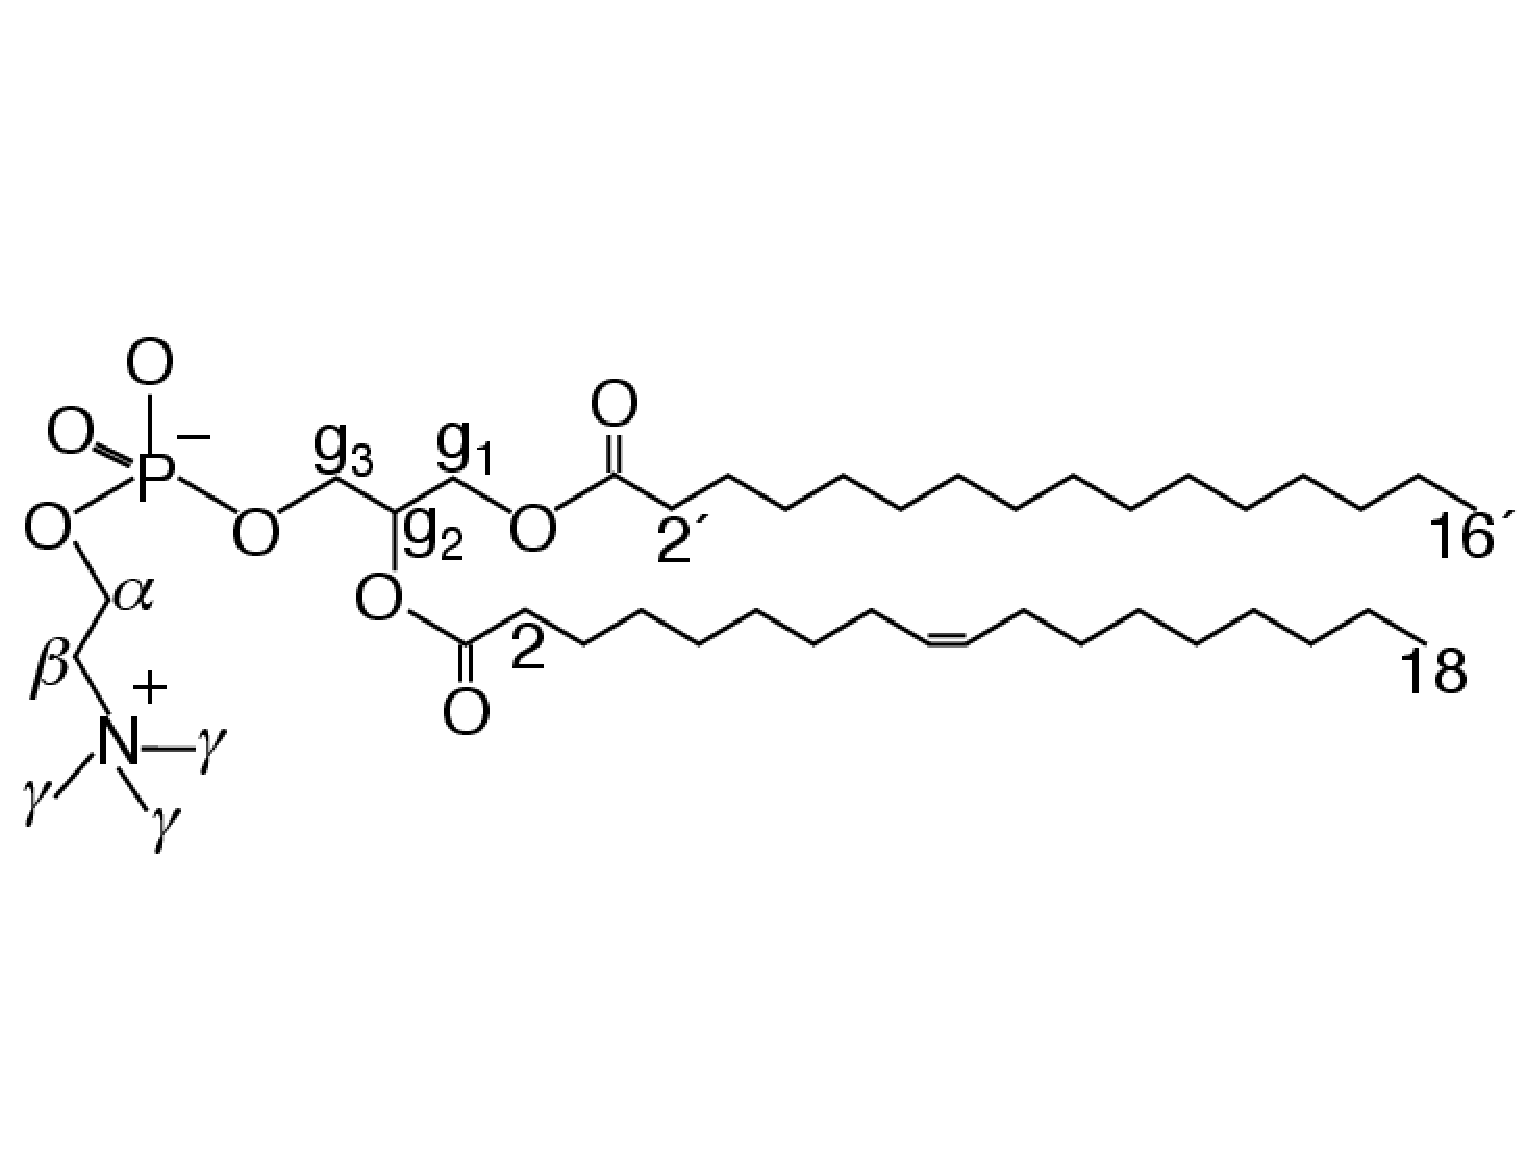
\includegraphics[width=8.6cm]{../Fig/POPCstructure.eps}

  \caption{\label{POPCstructure}
    Chemical structure of 1-palmitoyl-2-oleoylphosphatidylcholine (POPC).}
  
\end{figure}

\section{Results and Discussion}
The electrometer concept is originally based on the measured absolute value increase for $\beta$ 
and decrease for $\alpha$ segment order parameters with bound cations~\cite{akutsu81,altenbach84,seelig87,scherer89}.
However, the later experiments assigned negative sign for $\beta$ order parameter and positive for $\alpha$~\cite{hong95a,hong95b,gross97},
thus the both order parameter values are actually decreasing (becoming more negative) with bound
cations~\cite{ollila15}. The headgroup order parameters values from H$^2$ NMR~\cite{akutsu81,altenbach84}
together with correct signs~\cite{hong95a,hong95b,gross97} as a function NaCl and CaCl$_2$ concentrations
for DPPC and POPC bilayers are shown in Fig.~\ref{ordPions}. Only minute decrease is measured with 
NaCl while order of magnitude larger effect is observed with CaCl$_2$. Thus, according to the electrometer concept
monovalent Na$^+$ ion has negligible lipid bilayer affinity with these concentrations in constrast to multivalent 
Ca$^{2+}$ ions~\cite{akutsu81,altenbach84}. This conclusion is in agreement with several other experimental 
studies~\cite{cevc90,tocanne90,binder02,pabst07,filippov09}.
\begin{figure*}[]
  \centering
  \includegraphics[width=15cm]{../Fig/OrderParameterIONSchanges.eps}
  \caption{\label{ordPions}
    The order parameter changes for $\beta$ and $\alpha$ segments as a function of NaCl (left column) 
    and CaCl$_2$ (right column) concentrations from simulations and experiments~\cite{akutsu81} 
    (POPC with CaCl$_2$ from \cite{altenbach84}). The signs of the experimental order parameters, taken from
    experiments without ions~\cite{hong95a,hong95b,gross97}, can be assumed to be unchanged 
    with concentrations represented here~\cite{altenbach84,ollila15}. It should be noted that
    none of the models used here reproduces the order parameters within experimental error
    for pure PC bilayer wihtout ions, indicating structural inaccuracies with varying severity
    for all models \cite{botan15}.
   }
\end{figure*}

The headgroup order parameters in Fig.~\ref{ordPions} with added NaCl shows different behaviour for different simulation
models. The simulated systems are described in Table~\ref{IONsystems} and in Supplementary Information. 
While all simulation models show order parameter decrease due to Na$^+$ ion binding, 
significantly different binding affinities are predicted by different models.
This is demonstrated by plotting the density profiles from different models 
in increasing order according to the observed order parameters changes with NaCl concentration
in Fig.~\ref{NAdensities}. The Na$^+$ density peaks at the lipid bilayer interface clearly increase 
towards the bottom of the figure, thus correlating with the increased order parameter change. 
In conclusion, the choline structural response to the Na$^+$ binding is qualitatively correct 
and the electrometer concept~\cite{akutsu81,altenbach84,seelig87,scherer89} can be used to analyze the
Na$^+$ binding affinity in simulations, despite of the varying quality of the sampled choline and 
glycerol backbone structures in different simulation models~\cite{botan15}.
\begin{table*}[htb]
\centering
\caption{Simulated lipid bilayers with ions. The ion concentrations are the concentration of 
  ions in buffer to solute the lipid bilayers and calculated as [ion]=(N$_{\rm ion} \times$[water])/N$_{\rm w}$, 
  where [water]=55.5M. These correspond the concentrations reported in the experiments by Akutsu et al.~\cite{akutsu81}.
  The lipid force field parameters are denominated as in previous work~\cite{botan15}.
  For ion force field parameters the general force field for non--bonded parameters is mentioned and the citation to specific
  ion parameters is then given, if available.}\label{IONsystems}
\begin{tabular}{c c c c c c c c c c c c}
  %\hline
  Force field (lipid, ion)& lipid & [Ion] mM & \footnote{The number of lipid molecules}N$_{\rm l}$   &  \footnote{The number of water molecules}N$_{\rm w}$   & \footnote{The number of Na$^+$ molecules}N$_{\rm Na}$  & \footnote{The number of Ca$^{2+}$ molecules}N$_{\rm Ca}$   &  \footnote{The number of Cl molecules}N$_{\rm Cl}$ & \footnote{Simulation temperature}T (K)  & \footnote{The total simulation time}t$_{{\rm sim}}$(ns) & \footnote{Time frames used in the analysis}t$_{{\rm anal}}$ (ns) & Files\\
  \hline
  Berger-POPC-07\cite{ollila07a}   &   POPC & 0          & 128 & 7290 & 0  & 0  & 0 & 298  & 270 & 240 & \cite{bergerFILESpopc}  \\
  Berger-POPC-07\cite{ollila07a}, ffgmx\cite{straatsma88}  &   POPC & 340 (NaCl) & 128 & 7202 & 44  & 0  & 44 &298  & 110 & 50 & \cite{bergerPOPC340mMNaClfiles} \\
  %\hdashline
  Berger-POPC-07\cite{ollila07a}, ffgmx\cite{straatsma88}  &   POPC & 340 (CaCl$_2$) & 128 & 7157 & 0 & 44  & 88 &298 & 108 & 58 &\cite{bergerPOPC340mMCaClfiles}  \\
  \hline
  Berger-DPPC-98\cite{marrink98}   &   DPPC & 0 & 72 & 2880 & 0  & 0  & 0 &323  & 60 & 50 &\cite{bergerDPPCfiles} \\
  Berger-DPPC-98\cite{marrink98}, ffgmx\cite{straatsma88}   &   DPPC & 150 (NaCl) & 72 & 2880 & 8  & 0  & 8 &323  & 120 & 60 &\cite{bergerDPPC150mMfiles} \\
  Berger-DPPC-98\cite{marrink98}, ffgmx\cite{straatsma88}   &   DPPC & 1000 (NaCl) & 72 & 2778 & 51  & 0  & 51 &323  & 120 & 60 &\cite{bergerDPPC1000mMfiles} \\
  \hline
  BergerOPLS-DPPC-06\cite{tieleman06} &   DPPC & 0 & 72 & 2880 & 0  & 0  & 0 &323  & 120 & 60 &\cite{bergerOPLSDPPCfiles} \\
  BergerOPLS-DPPC-06\cite{tieleman06}, OPLS\cite{aqvist90} &   DPPC & 150 (NaCl) & 72 & 2880 & 8  & 0  & 8 &323  & 120 & 60 &\cite{bergerOPLSDPPCfiles150mMnacl} \\
  BergerOPLS-DPPC-06\cite{tieleman06}, OPLS\cite{aqvist90} &   DPPC & 1000 (NaCl) & 72 & 2778 & 51  & 0  & 51 &323  & 120 & 60 &\cite{bergerOPLSDPPCfiles1000mMnacl} \\
  \hline
  CHARMM36\cite{klauda10}   & POPC & 0           & 72 & 2242 & 0  & 0 & 0 & 303  & 30 & 20 & \cite{charmm36filesSHORT} \\
  CHARMM36\cite{klauda10}, CHARMM36\cite{venable13} & POPC & 350 (NaCl)  & 72 & 2085 & 13  & 0 & 13 & 303  & 80 & 60 & \cite{charmmPOPC350mMNaClfiles} \\
  CHARMM36\cite{klauda10}, CHARMM36\cite{venable13} & POPC & 690 (NaCl)  & 72 & 2085 & 26  & 0 & 26 & 303  & 73 & 60 & \cite{charmmPOPC690mMNaClfiles}   \\
  CHARMM36\cite{klauda10}, CHARMM36\cite{venable13}  & POPC & 950 (NaCl)  & 72 & 2168 & 37  & 0 & 37 & 303  & 80 & 60 &\cite{charmmPOPC950mMNaClfiles}  \\
  %CHARMM36\cite{klauda10}, ionFF~\cite{??}\todoi{Appropriate reference for the ion model?}  & POPC & 1380 (NaCl)  & 72 & 2085 & 52  & 0 & 52 & 303  & 80 & 60 &?\todoi{Samuli put to Zenodo} \\
  %CHARMM36\cite{klauda10}, ionFF~\cite{??}\todoi{Appropriate reference for the ion model?}   & POPC & 2080  (NaCl)  & 72 & 2085 & 78  & 0 & 78 & 303  & 73 & 60 &?\todoi{Samuli put to Zenodo} \\
  CHARMM36\cite{klauda10}, CHARMM36 & POPC &  350 (CaCl$_2$)  & 128 & 6400 & 0& 35 & 70 & 303  & 200  & 100 & \cite{charmmPOPC350mMCaClfiles}  \\
  CHARMM36\cite{klauda10}, CHARMM36 & POPC &  670 (CaCl$_2$)  & 128 & 6400 & 0& 67 & 134 & 303  & 200  & 120 & \cite{charmmPOPC670mMCaClfiles}  \\  
  CHARMM36\cite{klauda10}, CHARMM36 & POPC &  1000 (CaCl$_2$) & 128 & 6400 & 0& 100 & 200 & 303 & 200  & 100 & \cite{charmmPOPC1000mMCaClfiles}  \\
  \hline
  MacRog\cite{maciejewski14}  & POPC & 0 & 288 & 14400 & 0 & 0 & 0 & 310 & 90&40  &~\cite{macrogdehydFILES}  \\
  MacRog\cite{maciejewski14}, OPLS\cite{aqvist90}  & POPC & 100 (NaCl) & 288 & 14554 & 27 & 0 & 27 & 310 & 90&50  & \cite{macrogIONfiles} \\
  MacRog\cite{maciejewski14}, OPLS\cite{aqvist90}  & POPC &  210 (NaCl) & 288 & 14500 & 54 & 0 & 54 & 310 & 90&50  &\cite{macrogIONfiles}  \\
  MacRog\cite{maciejewski14}, OPLS\cite{aqvist90}  & POPC &   310 (NaCl) & 288 & 14446 & 81 & 0 & 81 & 310 & 90&50  & \cite{macrogIONfiles} \\
  MacRog\cite{maciejewski14}, OPLS\cite{aqvist90}  & POPC &   420 (NaCl) & 288 & 14392 & 108 & 0 & 108 & 310 & 90& 50  & \cite{macrogIONfiles}  \\
  \hline
  Orange, OPLS\cite{aqvist90}  &   POPC & 0 & 72 & 2880 & 0 & 0  & 0 & 298 & 60 & 50 & \cite{orangePOPCfiles}  \\
  Orange, OPLS\cite{aqvist90} &   POPC & 140 (NaCl) & 72 & 2866 & 7 & 0  & 7 & 298 & 120 & 100 &\cite{orangePOPC140mMNaClfiles}  \\
  Orange, OPLS\cite{aqvist90}  &   POPC & 510 (NaCl) & 72 & 2802 & 26 & 0  & 26 & 298 & 120 & 100 &\cite{orangePOPC510mMNaClfiles}   \\
  Orange, OPLS\cite{aqvist90}  &   POPC & 1000 (NaCl) & 72 & 2780 & 50 & 0  & 50 & 298 & 120 & 80 & \cite{orangePOPC1000mMNaClfiles} \\
  %\hdashline
  Orange, OPLS &   POPC & 510 (CaCl$_2$)  & 72 & 2802 & 0 & 26  & 52 & 298 & 120 & 60 & \cite{orangePOPC510mMCaClfiles}  \\
  \hline
  Slipid\cite{jambeck12}   &   DPPC & 0 & 128 &3840 & 0 & 0  & 0 & 323 & 150 & 100 &~\cite{slipidsFILES}  \\
  Slipid\cite{jambeck12}, AMBER\cite{beglov94,roux96} &   DPPC & 150 (NaCl) & 600 & 18000 & 49 & 0  & 49 & 323 & 100 & 40 &-  \\
  \hline
  Slipid\cite{jambeck12b}   &   POPC & 0 & 128 & 5120 & 0 & 0  & 0 & 303 & 200 & 150 &~\cite{slipidsFILESpopc}  \\
  Slipid\cite{jambeck12b}, AMBER\cite{smith94}  &  POPC & 130 (NaCl) & 200 & 9000 & 21 & 0  & 21 & 310 & 105 & 100 &~\cite{slipidsFILESpopc130mMnaclSD}  \\
  \hline
  Lipid14~\cite{dickson14}, AMBER\cite{aqvist90}  &   POPC & 0          & 128 & 5120 & 0 & 0  & 0 & 298 & 205 & 200 &~\cite{lipid14POPC0mMNaClfiles}  \\
  Lipid14~\cite{dickson14}, AMBER\cite{aqvist90}   &   POPC & 150 (NaCl) & 128 & 5120 & 12 & 0 & 12 & 298 & 205 & 200 &~\cite{lipid14POPC150mMNaClfiles}  \\
  Lipid14~\cite{dickson14}, AMBER\cite{aqvist90}   &   POPC & 1000 (NaCl) & 128 & 5120 & 77 & 0 & 77 & 298 & 205 & 200 &~\cite{lipid14POPC1000mMNaClfiles}  \\
  Lipid14~\cite{dickson14}, AMBER\cite{aqvist90}   &   POPC & 350 (CaCl$_2$) & 128 & 6400 & 0 & 35 & 70 & 298 & 200 & 100 &~\cite{lipid14POPC350mMCaClfiles}  \\
  Lipid14~\cite{dickson14}, AMBER\cite{aqvist90}   &   POPC & 1000 (CaCl$_2$) & 128 & 6400 & 0 & 100 & 200 & 298 & 200 & 100 &~\cite{lipid14POPC1000mMCaClfiles}  \\
  \hline
  Ulmschneiders~\cite{Ulmschneider09}, OPLS\cite{aqvist90}       &   POPC & 0          & 128 & 5120 & 0 & 0  & 0 & 298.15 & 205 & 200 &~\cite{ulmschneiderPOPC0mMNaClfiles}  \\
  Ulmschneiders~\cite{Ulmschneider09}, OPLS\cite{aqvist90}       &   POPC & 150 (NaCl) & 128 & 5120 & 12 & 0  & 12 & 298.15 & 205 & 200 &~\cite{ulmschneiderPOPC150mMNaClfiles}  \\
  Ulmschneiders~\cite{Ulmschneider09}, OPLS\cite{aqvist90}       &   POPC & 1000 (NaCl) & 128 & 5120 & 77 & 0  & 77 & 298.15 & 205 & 200 &~\cite{ulmschneiderPOPC1000mMNaClfiles}  \\
\end{tabular}
\end{table*} 
\begin{figure}[]
  \centering
  \includegraphics[width=8cm]{../Fig/NAdensities.eps}
  \caption{\label{NAdensities}
    Atom number density profiles along the membrane normal coordinate $z$ for lipids, Na$^+$ and Cl$^-$ ions from simulations with different force fields and different NaCl concetrations. 
    The force fields are ordered according to the order parameter changes observed in Fig.~\ref{ordPions} such that the models with smallest
    observed changes are top.
    The lipid densities are scaled with 100 (united atom) or 200 (all atom model) to make them visible with the used y-axis scale.
    Figure discussed in https://github.com/NMRLipids/lipid\_ionINTERACTION/issues/4.}
\end{figure}

The lowest Na$^+$ binding affinities and order parameter changes in best agreement with experiments are seen for the Orange,
CHARMM36 and Lipid14 models in Figs.~\ref{ordPions} and~\ref{NAdensities}. However, the ion density profiles in Fig.~\ref{NAdensities} show 
detectable differences in Na$^+$ affinity between these models, Orange having lowest affinity and CHARMM36 highest. 
With the achieved accuracy for the order parameters we are not able to conclude which of these three models has the most realistic 
Na$^+$ binding affinity, especially with physiological NaCl concentrations ($\sim$ 150mM) which is most relevant for most applications. 
%None of the models reproduces all the order parameters in Fig.~\ref{ordPions} within experimental error and 
%these very small order parameter changes (less than 0.02) may be delicate to, e.g. initial structures.
%Thus we cannot conclude if one of these three models is more realistic than another, 
On the other hand, the choline order parameter changes with NaCl are clearly overestimated in
all the other studied models indicating unrealistically strong Na$^+$ binding affinity to the bilayer.
This is manifested by the density peaks in Fig.~\ref{NAdensities}, seen also with physiological concentrations. 

The overestimated Na$^+$ binding may originate, e.g., from incorrect choline structure~\cite{botan15}, 
lack of polarizability~\cite{leontyev11}, other discrepancies in the ion models~\cite{hess06,chen07,Reif13} or from
combination of these and other issues. Interestingly, the same ion model and non--bonded parameters
are used in the Orange and BergerOPLS~\cite{tieleman06} simulations while Na$^+$ ion binding affinity
is realistic in the Orange model but overestimated in BergerOPLS model. This shows that the binding 
affinity significantly depends on the used lipid parameters. On the other hand, 
Na$^+$ binding with Berger, BergerOPLS and Slipid models is reduced but not yet agree with experiments 
by using the ion models with scaled charges to compensate the electronic polarizability~\cite{kohagen15,leontyev11}, 
see Supplementary Information. Further, Slipid model gives similar binding affinity with two different
ion parameters. These results indicate that at least lipid models need improvement to 
correctly predict the Na$^+$ binding affinity.

%The failure of Gromos ions to properly account ion--ion and ion--water binding propensities of Na$^+$ and Cl$^-$ ions has been
% reported previously~\cite{Reif13}. The \r{A}qvist ions have been parameterized in aqueous solutions with good agreement
% to experimental energies~\cite{Aaqvist90}. Yet, the binding affinity of ions to lipid bilayers has not been
% calibrated---instead it is assumed to work based purely on forces obtained using combination rules. Compared to Gromos
% ions, \r{A}qvist parameters are better, yet Na$^+$ overbinding still occurs.


%are arranged 
%such that the model with smallest change is on top and towards the bottom are models with larger observed order parameter changes.
%The order parameter decrease with penetrating cations is observed in all simulation models in line with experiments.
%This indicates that the 
%inaccuracies with varying severity in the choline and glycerol backbone structures, in agreement
%with our recent results with dehydration~\cite{botan15}.

%In our recent work, we showed that the experimental order parameters for choline and glycerol backbone were not
%quantitatively reproduced by any available lipid model in fully hydrated conditions, however, the response of the choline order parameters
%to dehydration were qualitatively correct in all 
%\todo{Markus: This 'all' gives the impression that it is the same as the 'any available' 
%in the beginning of the sentence. I propose we make it clear here that we only tested four FFs against dehydration.} 
%models, and the response to the cholesterol  content
%was qualitatively correct in the CHARMM36 model~\cite{botan15}. 
%\todo{Markus: Wouldn't you say that the response of the choline order parameters to cholesterol 
%content was qualitatively just as correct in MacRog as it was in CHARMM36? (Fig.~9 in Ref.~\cite{botan15})} 


%To study the correlation between order parameter changes and ion partitioning into a bilayer, 
%suggested by the electrometer concept~\cite{akutsu81,altenbach84,seelig87,scherer89}, the ion 
%density distributions from different simulation models as a function of membrane normal with NaCl and CaCl$_2$ are shown in 
%Figs.~\ref{NAdensities} and~\ref{CAdensitiesCLEAR}, respectively. 




\begin{figure}[]
  \centering
  \includegraphics[width=8cm]{../Fig/CAdensitiesCLEAR.eps}
  \caption{\label{CAdensitiesCLEAR}
    Atom number density profiles along the membrane normal coordinate $z$ for lipids, Ca$^{2+}$ and Cl$^-$ ions from simulations with different force fields.
    The profiles only with smallest available CaCl$_2$ concentration are shown for clarity.
    Figure including all the available concetrations is shown in the Supplementary Information.
    The lipid densities are scaled with 100 (united atom) or 200 (all atom model) to make them visible with the used y-axis scale.
    Figure discussed in https://github.com/NMRLipids/lipid\_ionINTERACTION/issues/4.
  }
\end{figure}
In contrast to Na$^+$, Ca$^{2+}$ binding and related order parameter decrease is seen in experiments~\cite{akutsu81,altenbach84,cevc90,tocanne90} 
and in all tested simulation models, see Figs. \ref{ordPions} and \ref{CAdensitiesCLEAR}.
While the significant Ca$^{2+}$ binding affinity to a phosphatidylcholine bilayer at mM concentrations  
is agreed in the literature, the estimations for lipid/Ca$^{2+}$ stoichiometry vary between 17 
and 0.24~\cite{tatulian87,altenbach84,bockmann04}. The smallest number (0.24) indicating that one 
Ca$^{2+}$ ion binds roughly four lipid molecules originates from simulation with Berger model~\cite{bockmann04}.
The direct comparison of order parameters between different simulation models and experiments in Fig.~\ref{ordPions}
shows that Ca$^{2+}$ binding induced changes are overestimated in all tested models.
In contrast to Na$^+$, clear correlation between Ca$^{2+}$ binding affinity and order parameter changes is not found, 
thus the overestimation of order parameter change may arise, e.g. from overestimated binding, 
incorrect headgroup response to penetrating divalent cation or penetration depth. 
The Berger model predicts deeper penetration depth (density maxima close to $\pm$1.8 nm) compared
to other models (density maxima close to $\pm$2 nm). The latter value is probably more realistic 
since $^1$H NMR and neutron scattering data indicates that Ca$^{2+}$ interact mainly with the 
choline group~\cite{hauser76,hauser78,herbette84,cevc90}.
Further, the $^1$H NMR experiments suggest that the N-$\beta$-$\alpha$-O dihedral is only in 
gaughe--conformation in the absense of ions, but in the presense of multivalent ions also anti--conformations
would be present \cite{hauser78, hauser81}. However, the glycerol backbone and headgroup atomistic resolution structures~\cite{botan15}
and their changes are not reproduced within experimental error in the tested simulation models,
thus the model development is needed before Ca$^{2+}$ binding affinity, lipid/ion stoichiometry 
and concomitant structural changes can be interpreted.
\todo{The P-N vector tilting analysis should be considered}
%I have now calculated the dihedral distributions for this dihedral with different CaCl$_2$ concentrations in different models, see Fig.~\ref{ObaNdihs}.
%The change suggested by the $^1$H NMR experiments is not seen in the CHARMM36 model. In Orange model this dihedral is mostly in anti
%conformation also without CaCl$_2$, oppositely as suggested by $^1$H NMR experiments. With CaCl$_2$ anti conformations become slightly more
%pronounced, however, the conformation seems to be unrealistic from the beginning so the studies of structural response to the CaCl$_2$
%might not be reasonable with this model. I think we need more simulations with CHARMM36 to see how good the order parameter response
%to the CaCl$_2$ actually is. Then we can discuss more about its structural response.} \\




%\begin{figure}[]
%  \centering
%  \includegraphics[width=8cm]{../Fig/OrderParameterIONSnaclSIGN.eps}
%  \caption{\label{ordPnacl}
%    Order parameters as a function of NaCl concentration from simulations 
%     with the Berger, CHARMM36, MacRog and Orange force fields compared to the experiments
%     by Akutsu et al.~\cite{akutsu81} and Altenbach et al.~\cite{altenbach84}. The signs are assumed to be the same as measured by Hong et al.~\cite{hong95a}, Hong et al.~\cite{hong95b} and Gross et al.~\cite{gross97}. 
%     The experimental data for the effect of ions to the glycerol backbone is not found, thus only the values without ions are shown. 
%     The straight line between the results with and without ions is plotted to guide the eye. 
%   }
%\todo{Samuli: I think that this figure could be removed. This is very unclear and I think would be difficult to make
%more clea. I am thinking that we could show the order parameters for pure bilayer compared to experiments 
%(as in the first paper) to remind the quality different models without ions. And the show only the changes
%as a function of ions. Issue discussed here: https://github.com/NMRLipids/lipid\_ionINTERACTION/issues/3
%
%Markus: Also, is there any point in showing the glycerol values as a function of [NaCl], if we do not have experimental data to compare against?}
%\end{figure}

%\begin{figure}[]
%  \centering
%  \includegraphics[width=8cm]{../Fig/OrderParameterIONSCaCl.eps}
%  \caption{\label{ordPcacl}
%    Order parameters as a function of CaCl concentration from simulations 
%     with the Berger 
%CHARMM36, MacRog 
%and Orange force fields compared to the experiments by Akutsu et al.~\cite{akutsu81} and Altenbach et al.~\cite{altenbach84}. 
%The signs are assumed to be the same as measured by Hong et al.~\cite{hong95a}, Hong et al.~\cite{hong95b} and Gross et al.~\cite{gross97}. 
%     The effect of ions to the g1 and g2 were not measured, thus only the values without ions are shown. The straight line between the results with and without ions is 
%     plotted to guide the eye. }
%\todo{I think that this figure could be removed as the previous. Issue discussed here: https://github.com/NMRLipids/lipid\_ionINTERACTION/issues/3}
%\end{figure}



%The most important observation is that the experimental order parameters for the headgroup and glycerol bakcbone g$_3$ segment 
%\todo{Markus: There seems to be NO experimental g$_3$ data in Fig.~\ref{ordPnacl}...}
%are practically unhanged even though 1M NaCl concentration was added to the system. Thus, the presence of mM concentrations
%of NaCl does not affect the structure of these parts of lipids. Thus, the most straightforward explanation for the experimental results shown
%in Fig.~\ref{ordPnacl} is that the Na$^+$ and Cl$^-$ ions do not essentially penetrate into a phospholipid bilayer below 1M concentrations.

%The response of order parameters to the NaCl concentration in simulations depends on the used model in Fig.~\ref{ordPnacl}:
%The addition of NaCl leads to a significant changes for choline and $g_2$ and g$_3$ segments in glycerol bakcbone
%in Berger and MacRog models, while only moderate changes are seen in CHARMM36 and Orange force fields.
%The experimental data for glycerol backbone as a function of NaCl concentration is available only for the
%g$_3$ segment. \todo{Markus: For some reason, these g$_3$ data are not shown in Fig.~\ref{ordPnacl}} 
%The changes in g$_1$ and g$_2$ are unlikely since all the other order parameters are unaffected
%and 

\section{Conclusions}
As suggested by the electrometer concept~\cite{akutsu81,altenbach84,seelig87,scherer89},
the headgroup $\alpha$ and $\beta$ segment order parameter decrease in phosphatidylcholine lipid bilayers 
is related to the cation binding affinity in all tested simulation models, despite of inaccuracies 
in actual atomistic resolution structures~\cite{botan15}. The concept allows direct comparison
of Na$^+$ binding affinity between simulations and NMR experiments by using the headgroup order parameter changes.
The comparison reveals that most models overestimate the Na$^+$ binding, only Orange, Lipid14 and CHARMM36 
predict realistic binding affinity. None of the tested models has the required accuracy to interpret
the Ca$^{2+}$/lipid stoichiometry or induced atomistic resolution structural changes.

In general the results support the traditional view that Na$^+$ and other monovalent ions (except Li$^+$)
do not specifically bind to the phospholipid bilayer with mM concetrations, in contrast to Ca$^{2+}$ and other multivalent 
ions~\cite{eisenberg79,akutsu81,altenbach84,tatulian87,clarke99,binder02,pabst07,filippov09}.
The contradicting results from molecular dynamics simulations~\cite{bockmann03,bockmann04}, fluorescent probe dynamics~\cite{bockmann03,vacha09a,harb13}, 
calorimetry~\cite{bockmann03,klasczyk10} and AFM~\cite{manyes05,manyes06,fukuma07,ferber11,morata12} suggesting stronger Na$^+$ binding can be explained by simulation artefacts, 
direct interactions between Na$^+$ and fluorescent probes~\cite{filippov09}, alternative intepretation of significance
of small phase transition temperature shift~\cite{cevc90} and insufficient resolution of AFM for atomistic resolution interpretation.

The artificial specific Na$^+$ binding in simulations may lead to duobtful results since it leads effectively 
positively charged phoshatidylcholine lipid bilayer even in physiological NaCl concetration.
Such a bilayer has distinctly different interactions with charged objects compared to the more realistic
model without specific Na$^+$ binding. Furthermore, the overestimation of Na$^+$ binding affinity may
extend also to other positively charged objects, e.g. membrane protein segments. This would affect
lipid protein interactions and could explain contradicting results on electrostatic interactions 
between charged protein segments and lipid bilayer \cite{arkhipov13,kaszuba15}. In conclusion, 
more careful studies and model development on lipid bilayer--charged object interactions are
needed to make molecular dynamics simulations straighforwardly usable in physiologically relevant
electrostatic environment. 


%The most straightforward explanation for our results is that Na$^+$ ions do not practically penetrate into a PC lipid bilayer
%at mM concentrations, thus the presense of NaCl does not affect the bilayer properties as observed in various 
%experiments~\cite{akutsu81,altenbach84,clarke99,binder02,pabst07,filippov09}.
%Consequently, the Na$^+$ penetration and concominant changes in order parameters, area per molecule and lateral diffusion 
%seen in almost all simulation models would be artefact due to overestimated attraction between ions and lipid bilayer.
%Even though this would also explain the absense of positive zeta potential in electrophoresis 
%experiments~\cite{eisenberg79,tatulian87,manyes05,manyes06,klasczyk10},  
%the presented data do not rule out the suggested possibility of equal binding of Na$^+$ and Cl$^-$ ions~\cite{knecht13},
%however, this equal binding should happen in such a way that the bilayer properties are unaffected.
%The negligible binding of Na$^+$ at mM concentrations suggested here differs from the conclusions made from 
%measurements of fluorescent probe dynamics~\cite{bockmann03,vacha09a,harb13}, membrane hardness with 
%AFM~\cite{manyes05,manyes06,fukuma07,ferber11,morata12} and calorimetry~\cite{bockmann03,klasczyk10}.
%However, the fluorescent measurement results may arise from direct interactions between probe and ions, as already 
%suggested by Filippov et al.~\cite{filippov09}. 
%Further, the calorimetric results have been also interpreted to support negligible binding~\cite{cevc90}, 
%and AFM result is relatively indirect, thus there may be alternative explanations as well.


%In conclusion, our results show that the Na$^+$ association to PC bilayer is significantly too strong in the Berger and MacRog models,
%while Orange and CHARMM36 force fields predict more realistic binding affinity. Since some modest changes are also seen in 
%Orange and CHARMM36 results, more careful simulation studies would be needed to judge if the Na$^+$ association is slightly 
%too strong also in these  models. The stonger Na$^+$ ion association in GROMOS based force fields compared to CHARMM based force 
%has been already reported in the literature~\cite{berkowitz06,cordomi09,valley11,berkowitz12,sachs04,valley11},
%however the novelty of this work in this respect is that we make a direct comparison
%to the experiments which can be used as measure for the model quality. 

%In situations where a positive charge penetrates into a bilayer (e.g. cationic surfactant~\cite{scherer89} or multivalent ion~\cite{akutsu81}) 
%a decrease in choline order parameters is observed in experiments, as also seen in CaCl$_2$ results in Fig.~\ref{ordPions}.
%Also in all simulations analyzed in this work where cation is penetrating into a bilayer, the choline order parameters
%decrease as seen in Fig.~\ref{ordPions}. However, in the case of CaCl$_2$ the decrease in too pronounced in 
%simulations which may arise from too strong partitioning of Ca$^{2+}$ or overestimated influence of charge on lipid conformation.



%Our discussion gives further support to the idea that choline orientation and ion partitioning can
%be experimentally measured by using the choline group order parameters as suggested in the series of
%publications by Seelig and co workers.
%However, we have updated the details of the relation by including the information about 
%the sings.

%- \todo{Final conclusions about the structural response to be written once we have all the results} 


%In conclusion, the penetrating induced decrease in order parameters can be seen in all models
%independently of the detailed molecular structure in the model, corresponding to the dehydration case
%where increase was seen in all models. The most likely explanation is that, despite of the structural model, the choline group
%orients more parallel to the membrane normal with penetrating cations. In contrast to the dehydration results,
%we are not aware of experimental data for the glycerol order parameters as a function of penetrating ions. 
%Furher, our results show that the Na$^+$ partitioning into a PC bilayer with Berger model is a
%simulation artefact, thus the research lines based these results should be taken with caution.


%This work has been done, and will be progressed, as an open collaboration through nmrlipids.blogspot.fi.






%Similar significant structural changes in the headgroup region are seen upon the addition
%of sodium and calcium ions in the Berger model. This contradicts with the experiments where
%sodium does not change the headgroup structure and the changes observed for calcium are different from those seen in simulations.
%These results indicate that the changes in the headgroup structure due to a permeating charge are not correct
%in the Berger model and, in particular, that sodium ions penetrating the headgroup region is erroneous.

This work has been, and will be, progressed and discussed through the blog: nmrlipids.blogspot.fi. 
Everyone is invited to join the discussion and make contributions through the blog. 
The manuscript will be eventually submitted to an appropriate scientific journal. 
Everyone who has contributed to the work through the blog will be offered 
coauthorship. For more details see: nmrlipids.blogspot.fi.   

{\bf Acknowledgements: }
OHSO acknowledges Tiago Ferreira for very useful discussions, the Emil Aaltonen foundation for financial support, Aalto Science-IT project and CSC-IT Center for Science for computational resources. 
%
MSM acknowledges financial support from the Volkswagen Foundation (86110).

\newpage

\appendix
\begin{center}
{\bf SUPPLEMENTARY INFORMATION}
\end{center}

\section{Effect of ion model and polarization}
It has been suggested that the missing electronic polarizability 
can be compensated by scaling the ion charge by a factor of 0.7 in 
simulations~\cite{leontyev11}. To test if this would improve the ion 
binding behaviour, we ran simulations with Berger-DPPC-98, BergerOPLS-DPPC-06
and Slipids with scaled Na$^+$ and Cl$^-$ ions. For Berger-DPPC-98 and BergerOPLS-DPPC-06 models 
the ion charge in systems listed in Table~\ref{IONsystems} was simply scaled with 0.7 and
the related files are available 
at ~\cite{DPPCBergerNaCl150mMscaled,DPPCBergerNaCl1000mMscaled,DPPCBergerOPLS06NaCl150mMscaled,DPPCBergerOPLS06NaCl1000mMscaled}). 
For simulations with Slipids the ion model by Kohagen et al. was used~\cite{kohagen15} and the simulation
details and related files are available at~\cite{slipidsFILESpopcSCALED}.
The order parameter changes and Na$^+$ binding affinity are decreased by the charge scaling but 
yet overestimated respect to the experiments as seen from Figs. \ref{OPchangesSCALED} and~\ref{NAdensitySCALED}. 
Thus the overestimated binding affinity cannot be fixed by only scaling charges.


%The intuitive explanation is that by scaling the partial charges the charge discrepancy between the ion and water partial charges is decreased. This means
%that there is a lesser driving force for ions to bind to the highly-charged phosphate group. Furthermore, with
%Berger-DPPC-06 and scaled \r{A}qvist ions (Q=0.7) we obtain that there is only very weak binding of sodium to DPPC as
%observed experimentally (right side of Figure \ref{ionscaled}). In scaled models the order parameter changes 
%are also small. However, the ion concentration is also small. To be fully conclusive, if the affinity can be fixed by scaling,
%we need to run simulations also with large concentrations.


%The results indicate that the polarization effect actually improves ion binding affinities irrespectively of the model.
%However, the drawback of the scaled charges is that the total charge of the simulation box is non-zero whenever
%counterions and charged molecules are present. This may cause simulation artefacts. Even though in methods such as
%PME the residual charge does not affect the forces (and thus dynamics), it still has an effect to the energies.
%This is because the potential from the residual charge is 'smeared in the box' and so depends on the possibly
%fluctuating (at least in NPT conditions) volume of the simulation box. 

\begin{figure}[]
  \centering
  \includegraphics[width=8cm]{../Fig/OrderParameterIONSchangesSCALED.eps} 
  \caption{\label{OPchangesSCALED}
    Order parameter changes in simulations using ion models with scaled charge. 
    }
\end{figure}

\begin{figure}[]
  \centering
  \includegraphics[width=8cm]{../Fig/NAdensitiesSCALED.eps} 
  \caption{\label{NAdensitySCALED}
    Atom number density profiles along membrane normal coordinate $z$ for lipids, Na$^+$ and Cl$^-$ ions from simulations using
    ion models with scaled charges. The lipid densities are scaled with 100 (united atom) or 200 (all atom model) to make them visible with the used y-axis scale.
}
\end{figure}


\section{Density distributions with different CaCl$_2$ concentrations}

The density distributions with all simulated CaCl$_2$ concentrations are shown in Fig.~\ref{CAdensities}.
\begin{figure}[]
  \centering
  \includegraphics[width=8cm]{../Fig/CAdensities.eps}
  \caption{\label{CAdensities}
    Number density profiles for lipids, Ca$^{2+}$ and Cl$^-$ ions from simulations with different force fields 
    and different CaCl$_2$ concentrations. 
    The lipid densities are scaled with 100 (united atom) or 200 (all atom model) to make them visible with the used y-axis scale.
    Figure discussed in https://github.com/NMRLipids/lipid\_ionINTERACTION/issues/4.
  }
\end{figure}


\section{methods}

\subsection{Simulated systems}
All simulations are ran with a standard setup for planar lipid bilayer in zero tension
with periodic boundary conditions with Gromacs software package (version numbers 4.5-X-5.0.X).

\subsection{Analysis}
The order parameters were calculated from simulation trajectories directly applying the equation
$S_{{\rm CH}}=\langle \frac{3}{2}  \cos^2 \theta-\frac{1}{2} \rangle$,
where $\theta$ is the angle between a given C--H bond and the bilayer normal and average is taken
over all lipids and timeframes. For united atom models the hydrogen locations
were regenerated for each molecule in each frame by using the {\it protonate} tool in 
Gromacs 4.0.2 \cite{gromacsMANUAL402}. For statistical error estimate order parameter
for each lipid molecule was separately calculated and the error of the mean over these 
values was used as done also in the previous work \cite{botan15}.
All the scripts used in analysis and the resulting data are available in the GitHub repository \cite{githubIONpaper}

\subsection{Simulation details}
\subsubsection{Berger}
{\it POPC} The simulation without ions is the same as in~\cite{ferreira13} and the files are available from~\cite{bergerFILESpopc}. 
The starting structures for simulations with ions is made by replacing water molecules with appropriate amount of ions.
The Berger force field was used for the POPC~\cite{berger97}, with the dihedral potential next to the double bond 
taken from~\cite{bachar04}. The ion parameters from ffmgx~\cite{straatsma88} were used.
Timestep of 2~fs was used with leap-frog integrator. Covalent bond lengths were constrained with LINCS algorithm~\cite{hess97,hess07}. 
Coordinates were written every 10~ps. PME~\cite{darden93,essman95} with real space cut-off 1.0~nm was used 
for electrostatics. Plain cut-off was used for the Lennard-Jones interactions with a 1.0~nm cut-off.
The neighbour list was updated every 5th step with cut-off 1.0~nm. Temperature was coupled separately
for lipids, water and ions to 298~K with the velocity-rescale method~\cite{bussi07} with coupling constant 0.1~ps$^{-1}$.
Pressure was semi-isotropically coupled to the athmospheric pressure with the Parrinello-Rahman barostat~\cite{parrinello81}.

{\it DPPC} The simulation without ions is the same as in~\cite{botan15} and the files are available from~\cite{bergerDPPCfiles}.
\todo{Simulation details from Jukka M{\"a}{\"a}tt{\"a}}

\subsubsection{BergerOPLS}
\todo{Simulation details from Jukka M{\"a}{\"a}tt{\"a}}

\subsubsection{CHARMM36}
{\it POPC with NaCl}
The simulation without ions is taken directly from~\cite{botan15,charmm36filesSHORT}. 
The starting structures for simulations with NaCl were made by replacing randomly located 
water molecules of the structure of pure POPC simulation with appropriate amount of ions.
The force field for lipid were the same as in~\cite{botan15,charmm36filesSHORT}.
The ion parameters with NBFIX by Venable et al.~\cite{venable13} were used.
Simulations were ran with Gromacs 4.5.5 software~\cite{pronk13}.
Timestep of 2~fs was used with leap-frog integrator. Covalent bonds with hydrogens were constrained with LINCS algorithm~\cite{hess97,hess07}. 
Coordinates were written every 5~ps. PME with real space cut-off 1.4~nm was used 
for electrostatics. Lennard-Jones interactions were switched to zero between 0.8~nm and 1.2~nm.
The neighbour list was updated every 5th step with cut-off 1.4~nm. Temperature was coupled separately
for lipids and solution to 303~K with the velocity-rescale method~\cite{bussi07} with coupling constant 0.2~ps.
Pressure was semi-isotropically coupled to the athmospheric pressure with the Berendsen method~\cite{berendsen84}.

%CaCl_2 simulations by MYKHAILO:
{\it POPC with CaCl$_2$}
The starting structures with varying amounts of CaCl$_2$ ions were constructed using the CHARMM-GUI Membrane Builder (http://www.charmm-gui.org/) online tool~\cite{lee15}. 
All runs were performed with Gromacs 5.0.3 software package~\cite{abraham15} and CHARMM36 additive force field parameters for lipids~\cite{klauda10} and ions were obtained from CHARMM-GUI input files. 
Standard CHARMM-GUI mdp options were used. Particularly, h-bond lengths were constrained with LINCS~\cite{hess97,hess07}. The temperatures of the 
lipids and the solvent were separately coupled to the Nose-Hoover~\cite{nose84,hoover85} thermostat with a target temperature of 303 K and a relaxation time constant of 1.0 ps. Semi-isotropical 
pressure coupling to 1 bar was obtained with the Parrinello-Rahman barostat~\cite{parrinello81} with a time constant of 5 ps. Equations of motion were integrated with the Verlet algorithm~\cite{pall13} 
using a timestep of 2 fs. Long-range electrostatic interactions were calculated using the PME~\cite{darden93,essman95} method with a fourth order smoothing spline. A real space cut-off of 1.2 nm 
was employed with grid spacing of 0.12 nm in the reciprocal space. Lennard-Jones interactions were smoothly swithced to zero between 1.0 nm and 1.2 nm. Verlet cutoff-scheme~\cite{pall13}  
were used with the long-range neighbor list updated every 20 steps. Coordinates were written every 10 ps.
After energy minimization and an equilibration run of 0.5 ns, 200ns simulations were ran and the last 100ns of each simulation was employed for the analysis.

\subsubsection{MacRog}
The simulation parameters are identical to those employed in our earlier study~\cite{botan15} for the full 
hydration and dehydration simulations. The initial structures with varying amounts of NaCl were constructed from an 
extensively hydrated bilayer by replacing water molecules with ions using the Gromacs tool genion~\cite{gromacsMANUAL}. Even at the highest 
considered salt concentration, the amount of water molecules per lipid after this replacement process was still greater than 50.

\subsubsection{Orange}
\todo{Jukka Maatta and Luca Monticelli, please deliver as much details as you can.}

\subsubsection{Slipids}
{\it DPPC} The simulation without ions from~\cite{botan15}, available at \cite{slipidsFILES} was used. 
For the simulations with ions, the starting DPPC lipid bilayer, which was built with the online CHARMM-GUI~\cite{lee15}
(http://www.charmm-gui.org/), contained 600 lipids, 30 water molecules/lipid, Na$^+$ and Cl$^-$ ions (150 mM NaCl). 
The TIP3P water model was used to solvate the system and ion parameters by Roux \cite{beglov94,roux96} were used. 
%All-atom MD simulations of DPPC lipid bilayers were performed 
%at ten different temperatures (283, 298, 303, 308, 312, 313, 314, 318, 323, and 333 K) using 
the GROMACS software  package version 4.5.5~\cite{pronk13} and the Stockholm lipids (Slipids) force field parameters 
for phospholipids were used. After energy 
minimization and a short equilibration run of 50 ps (time step 1~fs), 100 ns production runs were performed using 
a time step of 2~fs with leap-frog integrator. All covalent bonds were constrained with the LINCS~\cite{hess97,hess07}
algorithm. Coordinates were written every 100 ps. PME~\cite{darden93,essman95} with real space cut-off at 1.0 nm was used for Coulomb 
interactions. Lennard-Jones interactions were switched to zero between 1.0 nm and 1.4 nm. The neighbour 
lists were updated every 10$^\mathrm{th}$ step with a cut-off of 1.6 nm. Temperature was coupled separately for upper and 
bottom leaflets of the lipid bilayer, and for water to one of the temperatures reported above with the Nos\'e-Hoover 
thermostat~\cite{nose84,hoover85} using a time constant of 0.5 ps. Pressure was semi-isotropically coupled to the atmospheric pressure 
with the Parrinello-Rahman~\cite{parrinello81} barostat using a time constant of 10 ps.
%The last 40 ns of each simulation was employed for the analysis of DPPC choline and glycerol backbone order parameters.

{\it POPC} The simulation without ions from~\cite{botan15}, available at \cite{slipidsFILESpopc} was used. 
\todo{Simulation details for Slipids POPC simulation with ions from Matti Javanainen}

\subsubsection{Lipid14}
The starting structures with varying amounts of ions were constructed using the CHARMM-GUI Membrane Builder (http://www.charmm-gui.org/) 
online tool~\cite{lee15}. The GROMACS compatible force field parameters generated in~\cite{botan15} and 
available at~\cite{lipid14files} were used. 
The TIP3P water model~\cite{jorgensen83} was used to solvate the system and \r{A}qvist \cite{aqvist90} parameters were used for ions.
All runs were performed with Gromacs 5.0.3 software package~\cite{abraham15}
and LIPID14 force field parameters for POPC~\cite{dickson14}. 

H-bond lengths were constrained with LINCS~\cite{hess97,hess07}. The temperatures of the lipids and the solvent were separately coupled to the 
Nose-Hoover~\cite{nose84,hoover85} thermostat with a target temperature of 298.15 K and a relaxation time constant of 0.1 ps. Semi-isotropical pressure 
coupling to 1 bar was obtained with the Parrinello-Rahman barostat~\cite{parrinello81} with a time constant of 2 ps. Equations of motion were integrated 
with the Verlet algorithm~\cite{pall13} using a timestep of 2 fs. Long-range electrostatic interactions were calculated using the PME~\cite{darden93,essman95} method 
with a fourth order smoothing spline. A real space cut-off of 1.0 nm was employed with grid spacing of 0.12 nm in the reciprocal space. 
Lennard-Jones potentials were cut-off at 1 nm, with a dispersion correction applied to both energy and pressure. Verlet cutoff-scheme~\cite{pall13} 
were used with the long-range neighbor list updated every 20 steps. Coordinates were written every 10 ps.

After energy minimization and an equilibration run of 5 ns, 200ns production runs were performed and analysed. In case of the CaCl2 systems 
only the last 100ns of each simulation was employed for the analysis.

\subsubsection{Ulmscneiders}
The starting structures with varying amounts of ions were constructed using the CHARMM-GUI Membrane Builder (http://www.charmm-gui.org/) 
online tool~\cite{lee15}. The force field parameters were obtained from Lipidbook~\cite{domanski10}. The TIP3P water model~\cite{jorgensen83} 
was used to solvate the system.  Additionally, the simulations of ion-free bilayer were repeated with both Verlet and Group cutoff-schemes~\cite{ulmschneiderPOPC0mMNaClfiles}. 
There was no significant difference in headgroup or glycerol backbone order parameters between these cutoff-schemes. All runs were performed with Gromacs 5.0.3 software package~\cite{abraham15}. 
The glycerol backbone order parameters without iones were not the same as reported in the previous study~\cite{botan15}.
The origin of discrepancy was located to the different initial structures which was taken from CHARMM-GUI in this work
and from Lipidbook in the previous work. Since the order parameters with the initial structure from CHARMM-GUI are
closer to the experimental values, the results indicate that the structure available from Lipidbook is stuck to a
state with incorrect glycerol backbone strucuture, for more discussion see \url{https://github.com/NMRLipids/lipid_ionINTERACTION/issues/8}.

All-bond lengths were constrained with LINCS~\cite{hess97,hess07}. The temperatures of the lipids and the solvent were separately coupled to the Nose-Hoover~\cite{nose84,hoover85} 
thermostat with a target temperature of 298.15 K and a relaxation time constant of 0.1 ps. Semi-isotropical pressure coupling to 1 bar was obtained 
with the Parrinello-Rahman barostat~\cite{parrinello81} with a time constant of 2 ps. Equations of motion were integrated with the Verlet algorithm~\cite{pall13} using a 
timestep of 2 fs. Long-range electrostatic interactions were calculated using the PME~\cite{darden93,essman95} method with a fourth order smoothing spline. 
A real space cut-off of 1.0 nm was employed with grid spacing of 0.12 nm in the reciprocal space. Lennard-Jones potentials were cut-off at 1 nm, 
with a dispersion correction applied to both energy and pressure. Verlet cutoff-scheme~\cite{pall13} were used with the long-range neighbor list updated 
every 20 steps. Coordinates were written every 10 ps. After energy minimization and an equilibration run of 5 ns, 200ns simulations were ran and 
the last 100ns of each simulation was employed for the analysis.



\section{Author Contributions}
\noindent 
{\it Andrea Catte} \\
{\it Mykhailo Girych} \\
{\it Matti Javanainen} \\
{\it Markus S. Miettinen} \\
{\it Luca Monticelli}  \\
{\it Jukka M{\"a}{\"a}tt{\"a}}  \\
{\it Vasily S. Oganesyan} \\
{\it O. H. Samuli Ollila} co-designed the project with MSM and managed the work. Ran and analyzed several simulations. Wrote the manuscript. \\


%\onecolumngrid
\listoftodos

\bibliographystyle{apsrev}
\bibliography{refs}


\end{document}
